\documentclass{article}

\usepackage{amsmath}
\usepackage{amssymb}
\usepackage{minted}
\usepackage{graphicx}

\author{Austin Chase Minor}
\title{Cryptographic Applications of Random Variables}
\date{\today}

\begin{document}
   \maketitle

   \section{Introduction}
   You are a budding cryptanalyst and have noticed a security
   flaw in your companies login system. You find that matching
   certain keys to values gives you access to peoples' accounts.
   You have no way of determining which key/value pairs match.
   Also, you only have so many retry counts. 
   Your job is to determine the number of key/value matches you
   will get given a certain retry count. This is a mathematical
   hard problem to determine the exact probability of success. This
   is due to the fact that
   as a key/value is matched. The number of keys decrease, and thus
   the probability increases for a match. So remembering the theory
   of random variables, you deicide code the problem statement and simulate
   to find the average number of matches for a given retry count.

   We will start with the mathematical description of the problem.
   From there, we will give the problem statement. After running the
   test, we will analyze the problem and give a conclusion.

   \section{Mathematical Description}
   \begin{flushleft}
      Let $A, B$ be a set of keys and values respectively.\\
      Let $f: A \to B$ be the function relating
      keys to values that you are trying to discover.\\
      Let $\phi: A \times B \to {0,1}$ be a truth
      function representing $true = 1$ if $f(a) = b; a \in A, b \in B$
      and $false = 0$ otherwise.\\
      Let $k \in \mathbb{N}$ represent the
      number of retry counts allowed (the number of tries for each individual
      $b \in B$ to the $\phi$ function.\\
   \end{flushleft}

   \section{Problem Statement}
      Through some thought, it can be shown that the best way to go
      about trying potential values is to try each $b \in B$ with
      every $a \in A$ $k$ times removing $a$'s as they are matched
      according to the $\phi$ function. This
      guarantees a minimum of $k$ matches. Furthermore, it maximizes the
      shared information between $a$'s resulting in a higher probability.
      This is intuitively seen by noticing that every time an $b$ is tried
      against a $a$ the probability of of not succeeding decreases.

      By repeating this trial over k several times, we can generate
      a sample of the actual probability. This allows us to estimate
      the mean and standard deviation along with seeing the general
      shape of the function. The Matlab code for this along with
      the corresponding graphs are below.

      \begin{listing}[H]
         \inputminted[linenos]{matlab}{../../crypto_sim.m}
         \caption{CryptoSim Main}
      \end{listing}
      \begin{listing}[H]
         \inputminted[linenos]{matlab}{../../match.m}
         \caption{Match}
      \end{listing}
      \begin{listing}[H]
         \inputminted[linenos]{matlab}{../../randomize_array.m}
         \caption{Randomize Array}
      \end{listing}
   \section{Analysis of Problem}
      \begin{figure}[H]
         \includegraphics[width=\textheight/2]{images/3d_matches.png}
         \caption{3D Image of the match frequences and numbers}
      \end{figure}
      \begin{figure}[H]
         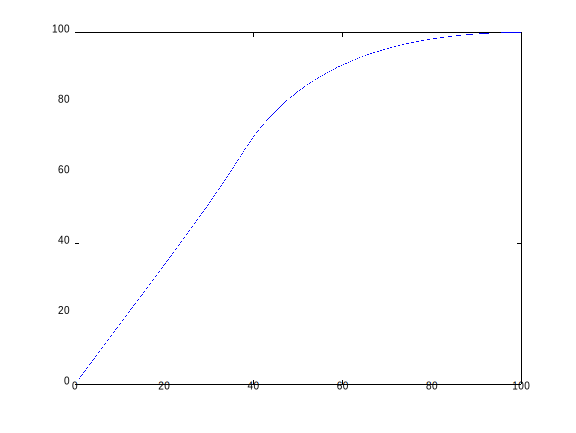
\includegraphics[width=\textheight/2]{images/mean.png}
         \caption{Average mathches over k --
                  matches - y-axis; k - x-axis}
      \end{figure}
      \begin{figure}[H]
         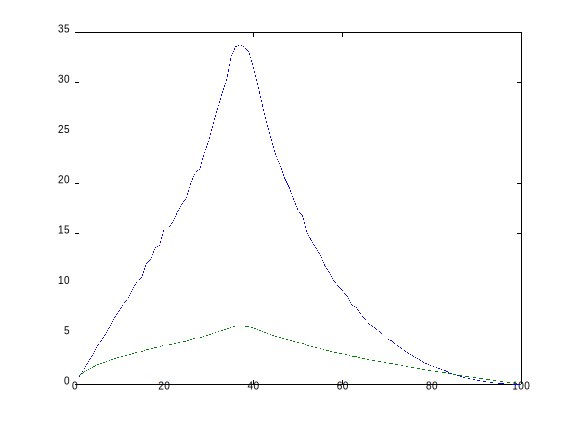
\includegraphics[width=\textheight/2]{images/dev_var.png}
         \caption{Standard Deviation and Variance over k --
                  Standard Deviation - green; Variance - blue}
      \end{figure}

      It is logical to assume that at a certain point k their would
      be a tipping point. I.E. their would be a point where the number
      of matches being found would reduce the number left to find in a
      vicious cycle resulting in complete matches at a lower number.
      However, Figure 2 shows that this indeed is not
      what happens. Instead the graph increases linearly then levels
      off. This is surprising and means that in theory this problem
      is not as insecure as it may seem at first glance. Other
      than that, the mean shows that the
      number of matches to k is between (1:1 and 2:1). We have no theory
      for why the average matches level out instead of jumping to 100\%.
      Further research needs to be done to determine a mathematical model of the
      problem to see why this is the case since it is not expected intuitively.

      Overall, the matches you receive are fairly consistent. This is
      shown by the standard deviation in Figure 3. At max, the standard
      deviation is 5-6. This occurs around 38. We theorize that this is
      due to the leveling off of the graph in Figure 2 for high k. We theorize
      that for low k this
      is due to the lack of matches contributing to more matches,
      this phenomenon being described above. Thus
      according to Figure 3, an attacker would be
      able to consistently break the system at the rate given by Figure 2 (the mean).
   \section{Conclusion}
      We discovered that this problem is far from being as cryptographically
      insecure as at first glance. The growth rate does not hit a tipping
      point. Rather, it actually levels off instead. Further investigation
      is needed to understand why this happens. This phenomenon
      moves the problem down from a high security problem
      to a medium security problem since their is not a tipping point for
      gaining 100\% matches.
\end{document}
